\documentclass[11pt, letterpaper]{article}
\usepackage[margin=0.75in]{geometry}
\usepackage{enumitem, amsmath, booktabs, graphicx, xcolor}
\pagestyle{empty}

\begin{document}

\begin{center}
{\Large\bfseries Conference Slide Content}\\[6pt]
{\large Volatility Input Choice and Delta Hedging Performance: Evidence from SPX Options}\\[4pt]
{\normalsize Zaid Annigeri --- Future Alpha 2026}
\end{center}

\vspace{0.5em}
\noindent\rule{\textwidth}{0.8pt}

% ═══════════════════════════════════════════════════════════
\section{Slide 1: Title}

\subsection*{On-Slide Content}
\begin{itemize}[nosep]
  \item \textbf{Volatility Input Choice and Delta Hedging Performance:}\\
        \textbf{Evidence from SPX Options}
  \item Zaid Annigeri \quad|\quad Master of Quantitative Finance, Rutgers Business School
  \item Future Alpha 2026 \quad|\quad March 31--April 1, Brooklyn Marriott
\end{itemize}

\subsection*{Figure}
None (title slide).

\subsection*{Speaker Notes}
Good morning. I'm Zaid, an MQF student at Rutgers Business School. My thesis asks a simple question that every options desk faces daily: which volatility should you use to compute your hedge ratios? The textbook says implied vol, practitioners often prefer realized vol, and surface models like SVI promise more precision. I tested five different answers on real SPX options over six years. The results were surprising---the simplest estimator wins, and the most sophisticated one actually hurts. Let me show you why.

\noindent\rule{\textwidth}{0.4pt}

% ═══════════════════════════════════════════════════════════
\section{Slide 2: The Problem}

\subsection*{On-Slide Content}
\begin{itemize}[nosep]
  \item Every day, options desks choose a volatility to compute hedge ratios.
  \item 5 candidates: Flat BSM IV, SVI Surface IV, Close-to-Close RV, Parkinson RV, Yang-Zhang RV
  \item Which one actually minimizes hedging error?
\end{itemize}

\subsection*{Figure}
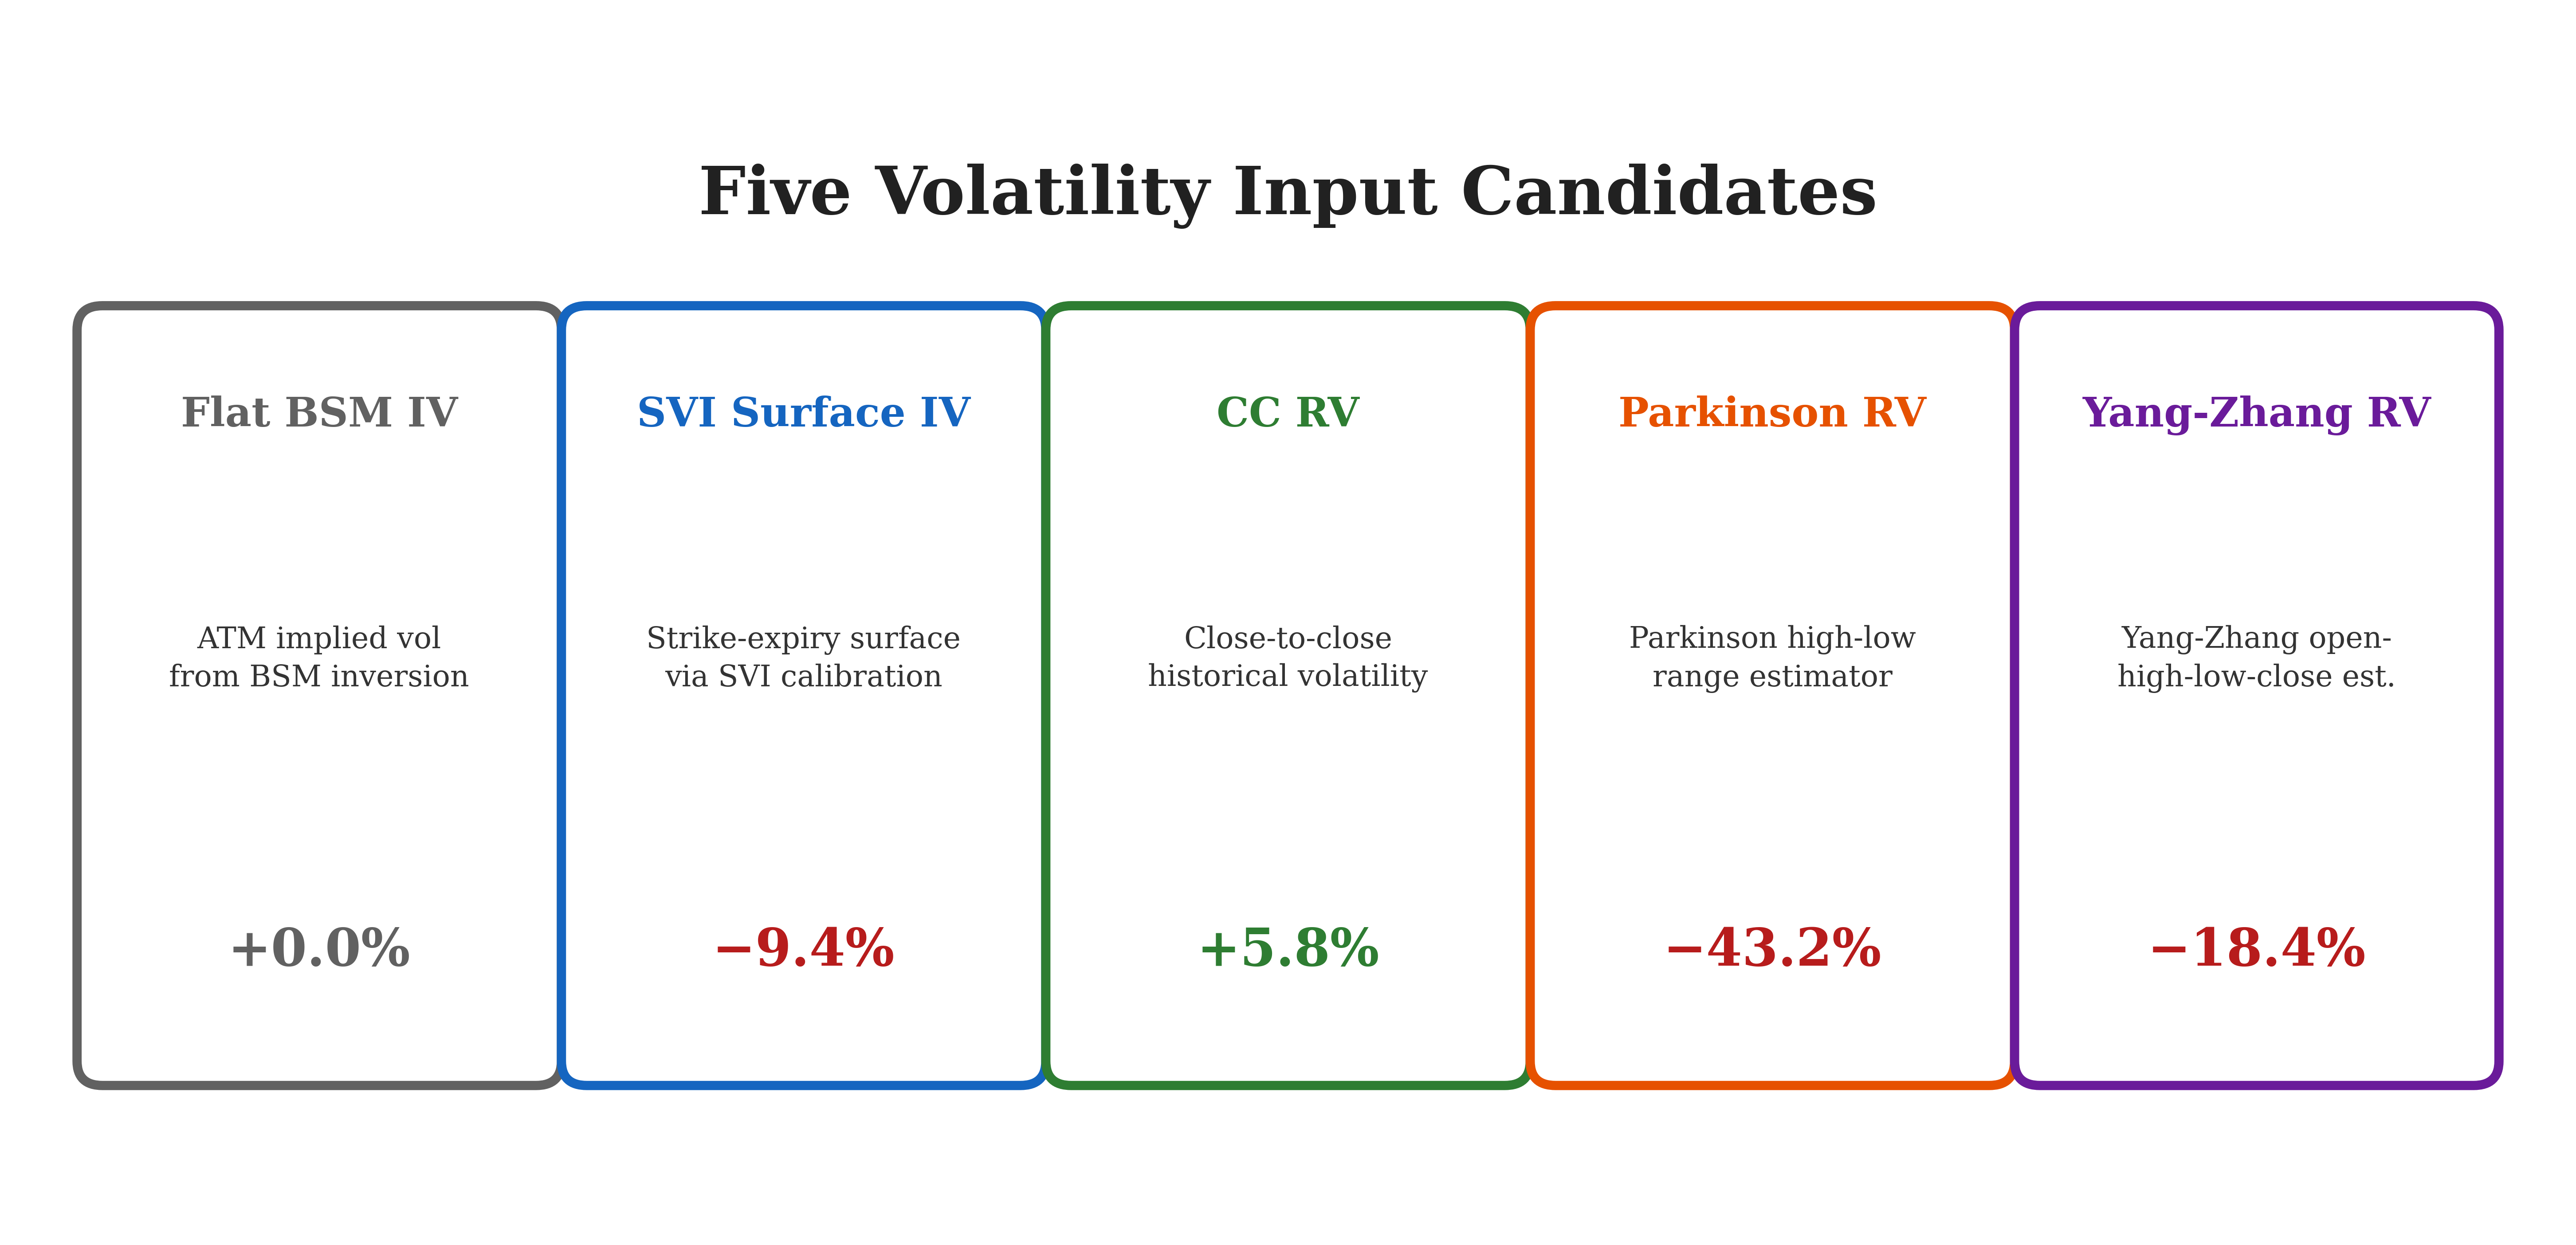
\includegraphics[width=0.85\textwidth]{fig_vol_choice_visual.png}

\subsection*{Speaker Notes}
Think about an options desk. Every morning, they need to decide: do I hedge with the ATM implied vol? The full volatility smile? Or some estimate of what vol has actually been? The wrong choice shows up as unexplained P\&L. There are five natural candidates, ranging from the simplest flat implied vol to a calibrated SVI surface and three different realized vol estimators that use different amounts of intraday information. I tested all five head-to-head on identical options with identical rebalancing. The only thing that changes is the sigma feeding into the delta formula.

\noindent\rule{\textwidth}{0.4pt}

% ═══════════════════════════════════════════════════════════
\section{Slide 3: The Gap}

\subsection*{On-Slide Content}
\begin{itemize}[nosep]
  \item SVI is the industry standard for volatility surface calibration.
  \item Extensive literature validates calibration quality (10--50 bps RMSE).
  \item But: does a better surface fit $\Rightarrow$ better hedging?
  \item[] \textbf{\Large Nobody has tested this.}
\end{itemize}

\subsection*{Figure}
None (text slide).

\subsection*{Speaker Notes}
SVI---Stochastic Volatility Inspired---is what most desks use to fit the implied volatility smile. There is a huge literature showing it fits well, with RMSEs in the 10 to 50 basis point range. Gatheral, Jacquier, De Marco---all focused on calibration quality. But fitting well and hedging well are different things. Fitting captures the cross-sectional shape of the smile at one moment; hedging requires that shape to carry forward-looking information about how delta should change. No one had actually closed the loop and tested whether better SVI fits produce better hedge ratios. That is the gap this thesis fills.

\noindent\rule{\textwidth}{0.4pt}

% ═══════════════════════════════════════════════════════════
\section{Slide 4: Data \& Sample}

\subsection*{On-Slide Content}
\begin{itemize}[nosep]
  \item S\&P 500 options, January 2019 -- December 2024
  \item 28.6M raw $\rightarrow$ 5.6M filtered $\rightarrow$ 2{,}000 stratified sample
  \item 500 options per VIX regime: Low $\cdot$ Normal $\cdot$ High $\cdot$ Crisis
  \item Covers: COVID crash (VIX 82.7), 2022 rate hikes, 2023--24 normalization
\end{itemize}

\subsection*{Figure}
\includegraphics[width=0.85\textwidth]{../figures/fig1_spx_vix_regimes.png}

\subsection*{Speaker Notes}
I used OptionMetrics data---the gold standard for academic options research. Six years spanning everything from the COVID crash, where VIX hit 82.7, to the 2022 rate hiking cycle, through the 2023--2024 normalization. I stratified my sample so I have exactly 500 options per VIX regime, giving equal representation across calm and crisis periods. This avoids results being dominated by any single market environment. The figure shows SPX and VIX with the regime classification---you can see the four distinct environments that the sample covers.

\noindent\rule{\textwidth}{0.4pt}

% ═══════════════════════════════════════════════════════════
\section{Slide 5: Methodology}

\subsection*{On-Slide Content}
\begin{itemize}[nosep]
  \item Daily BSM delta hedge: sell option, hedge to expiry
  \item Delta: $\Delta = e^{-qT}N(d_1)$, computed with each $\sigma_h$
  \item SVI calibration: Gatheral raw SVI, 3-stage optimizer (LS $\rightarrow$ DE $\rightarrow$ L-BFGS-B)
  \item El Karoui P\&L decomposition: discrete rebalancing + vol misspecification + higher-order residual
  \item Gain statistic: $\text{Gain} = 1 - \sigma_h / \sigma_{\text{BSM}}$ (Hull \& White, 2017)
\end{itemize}

\subsection*{Figure}
None (equations slide).

\subsection*{Speaker Notes}
The protocol is straightforward. Sell an option, delta-hedge it daily to expiry, and measure the hedging error---the difference between the option payoff and the accumulated hedge portfolio. Do this with each of the five volatility inputs, so the only thing that changes is the sigma feeding into the BSM delta formula. The SVI calibration uses a three-stage optimizer: least-squares initialization, differential evolution for global search, and L-BFGS-B for local refinement. Then I decompose the P\&L using El Karoui's framework, which separates the hedging error into three sources: discrete rebalancing, volatility misspecification, and a residual capturing vanna, volga, and jumps. The Gain statistic from Hull and White measures percentage reduction in hedging error standard deviation.

\noindent\rule{\textwidth}{0.4pt}

% ═══════════════════════════════════════════════════════════
\section{Slide 6: SVI Calibration Quality}

\subsection*{On-Slide Content}
\begin{itemize}[nosep]
  \item 19.5 bps median RMSE across 3{,}069 calibrated slices
  \item 98\% convergence rate
  \item 68.6\% Durrleman butterfly arbitrage-free (82.4\% for RMSE $<$ 25 bps)
  \item Competitive with industry-grade implementations
\end{itemize}

\subsection*{Figure}
\includegraphics[width=0.85\textwidth]{../figures/fig3_svi_fit_examples.png}

\subsection*{Speaker Notes}
Before we get to hedging results, let me show you that the SVI calibration works well. Median RMSE of 19.5 basis points---that is competitive with industry-grade implementations. I calibrated 3,069 expiry slices using the three-stage optimization. 68.6\% of slices pass the Durrleman butterfly arbitrage check, and for the best-fit slices under 25 basis points RMSE, that rate jumps to 82.4\%. The figure shows representative fits across different regimes. These fits look good. The question is whether good fits translate to good hedging. Spoiler: they do not.

\noindent\rule{\textwidth}{0.4pt}

% ═══════════════════════════════════════════════════════════
\section{Slide 7: The Main Result}

\subsection*{On-Slide Content}
\begin{itemize}[nosep]
  \item Results summary (Std of hedging error, Gain vs.\ Flat BSM):
  \begin{itemize}[nosep]
    \item[\textcolor{green!60!black}{$\blacktriangledown$}] RV Close-Close: Std = \$39.66, Gain = \textbf{+5.8\%} ($p = 0.008$)
    \item Flat BSM: Std = \$42.10 (baseline)
    \item[\textcolor{red!70!black}{$\blacktriangle$}] SVI Surface: Std = \$46.04, Gain = \textbf{$-$9.4\%} ($p < 0.001$)
    \item RV Yang-Zhang: Std = \$49.86, Gain = $-$18.4\%
    \item RV Parkinson: Std = \$60.30, Gain = $-$43.2\%
  \end{itemize}
  \item \textbf{The simplest estimator wins. The most complex surface hurts.}
\end{itemize}

\subsection*{Figure}
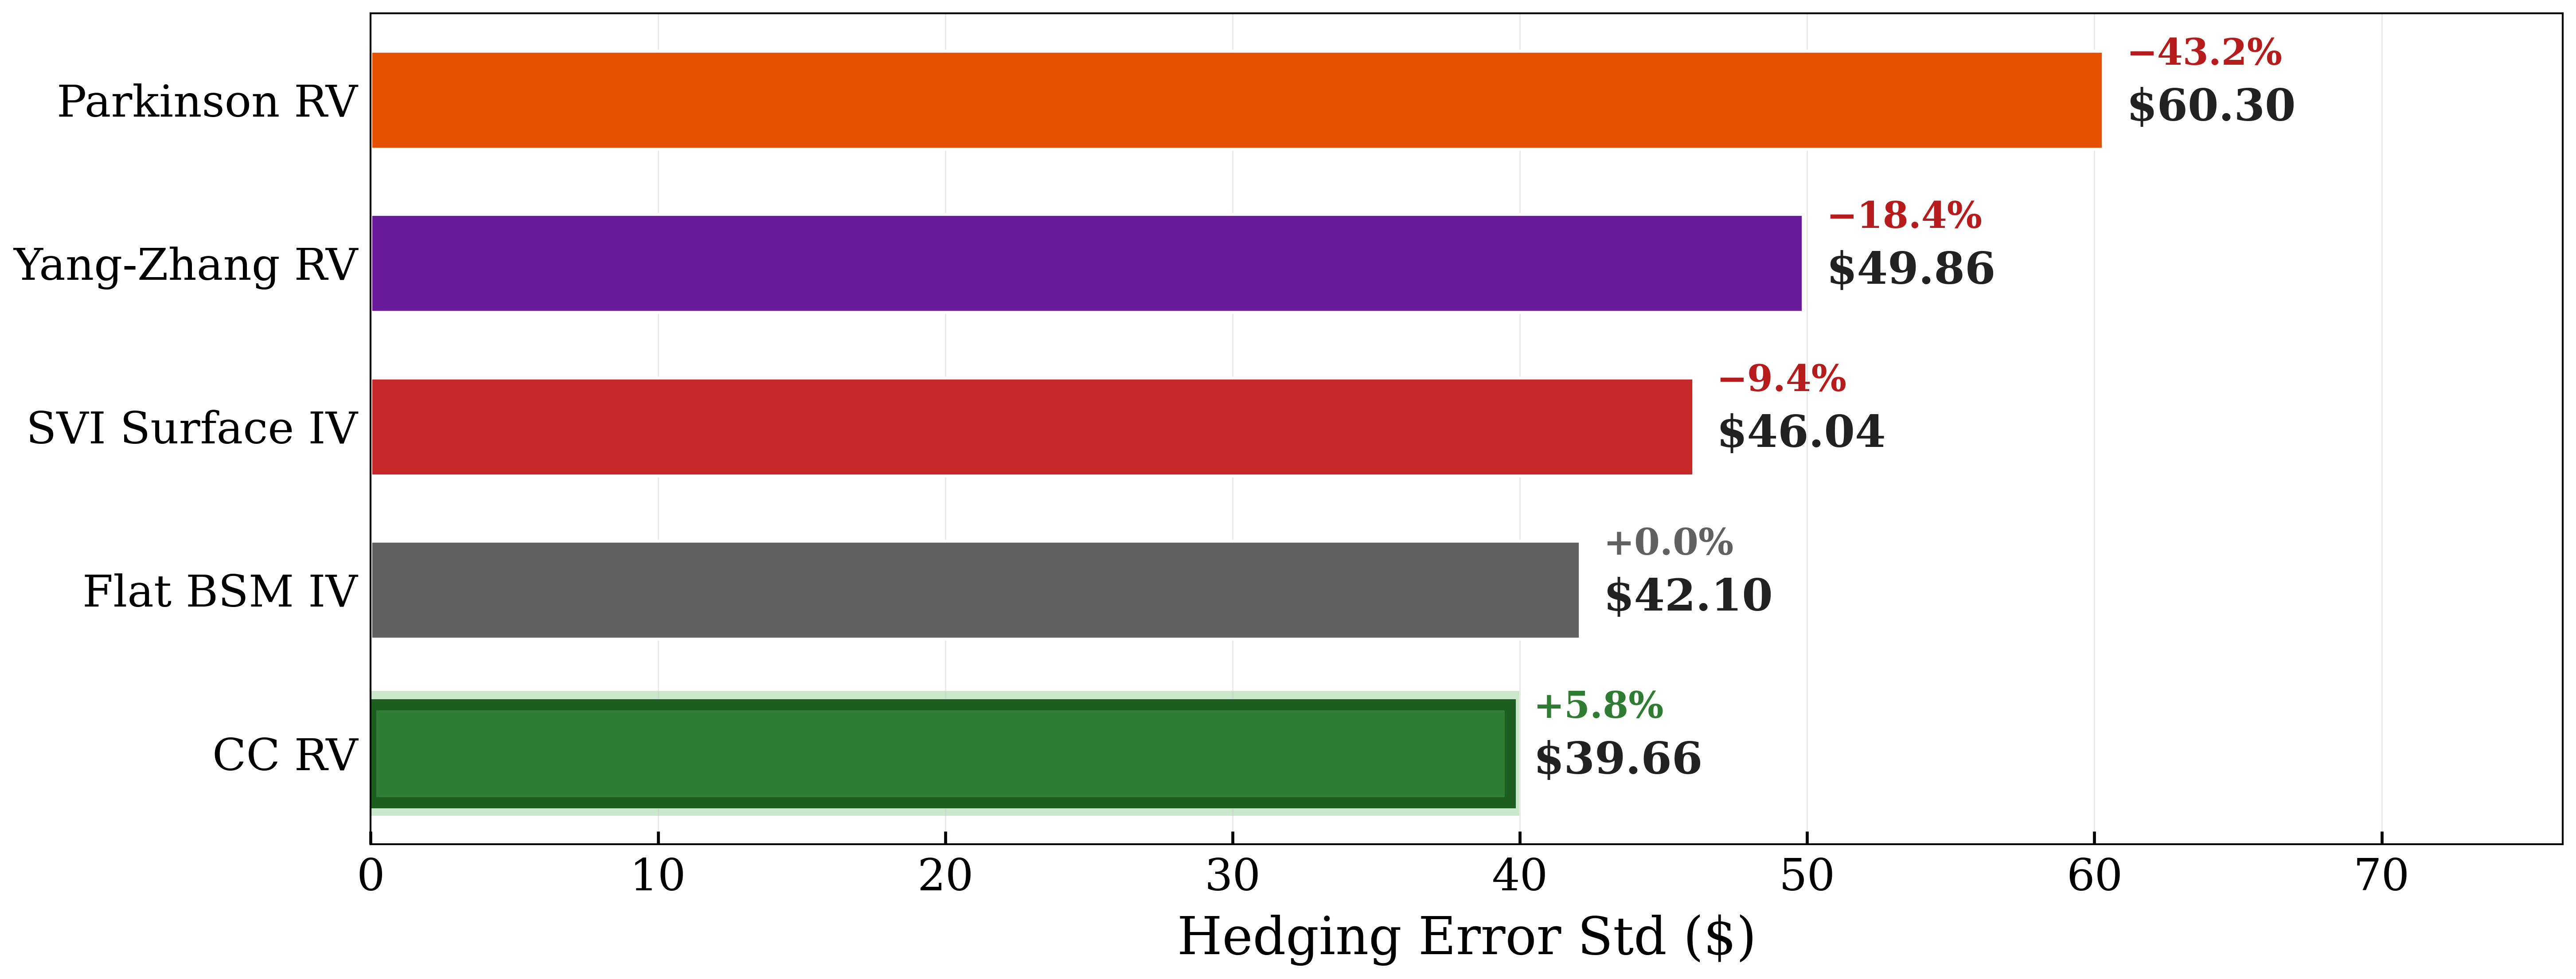
\includegraphics[width=0.85\textwidth]{fig_results_highlighted.png}

\subsection*{Speaker Notes}
And here is the surprise. This is the key slide. Close-to-close realized vol---the simplest estimator, using only closing prices---reduces hedging error standard deviation by 5.8\% relative to flat BSM. That is statistically significant at $p = 0.008$. But SVI, despite all that calibration work, actually makes hedging worse by 9.4\%, significant at $p < 0.001$. More information does not mean better hedging. The volatility surface adds calibration noise that outweighs the information content of the smile for most strikes. Parkinson and Yang-Zhang are even worse---their sensitivity to intraday prices is a liability for hedging, not an advantage.

\noindent\rule{\textwidth}{0.4pt}

% ═══════════════════════════════════════════════════════════
\section{Slide 8: The Twist --- Moneyness Matters}

\subsection*{On-Slide Content}
\begin{itemize}[nosep]
  \item SVI wins for OTM calls: +6--12\% RMSE reduction
  \item CC wins for OTM puts: +21--48\% RMSE reduction
  \item Flat BSM wins for ATM short-dated
  \item No single input wins everywhere
\end{itemize}

\subsection*{Figure}
\includegraphics[width=0.85\textwidth]{../handout/fig_moneyness_heatmap.png}

\subsection*{Speaker Notes}
But here is where it gets interesting. When I break results down by moneyness and time to expiry, the picture flips. SVI actually wins for out-of-the-money calls---where the smile slope is steepest and carries real information about delta. Close-to-close realized vol wins for OTM puts, where the skew premium makes implied-vol-based deltas systematically biased. And for ATM options with short maturities, flat BSM is fine because the smile is nearly flat anyway. The heatmap shows which input wins in each moneyness-by-DTE cell. No single volatility input wins everywhere---which motivates a conditional strategy.

\noindent\rule{\textwidth}{0.4pt}

% ═══════════════════════════════════════════════════════════
\section{Slide 9: P\&L Attribution}

\subsection*{On-Slide Content}
\begin{itemize}[nosep]
  \item Higher-order residuals dominate across ALL regimes (150--210\%)
  \item Discrete rebalancing error is negatively correlated with total P\&L
  \item Gamma exposure is the common driver
  \item Implication: gamma management $>$ volatility input choice
\end{itemize}

\subsection*{Figure}
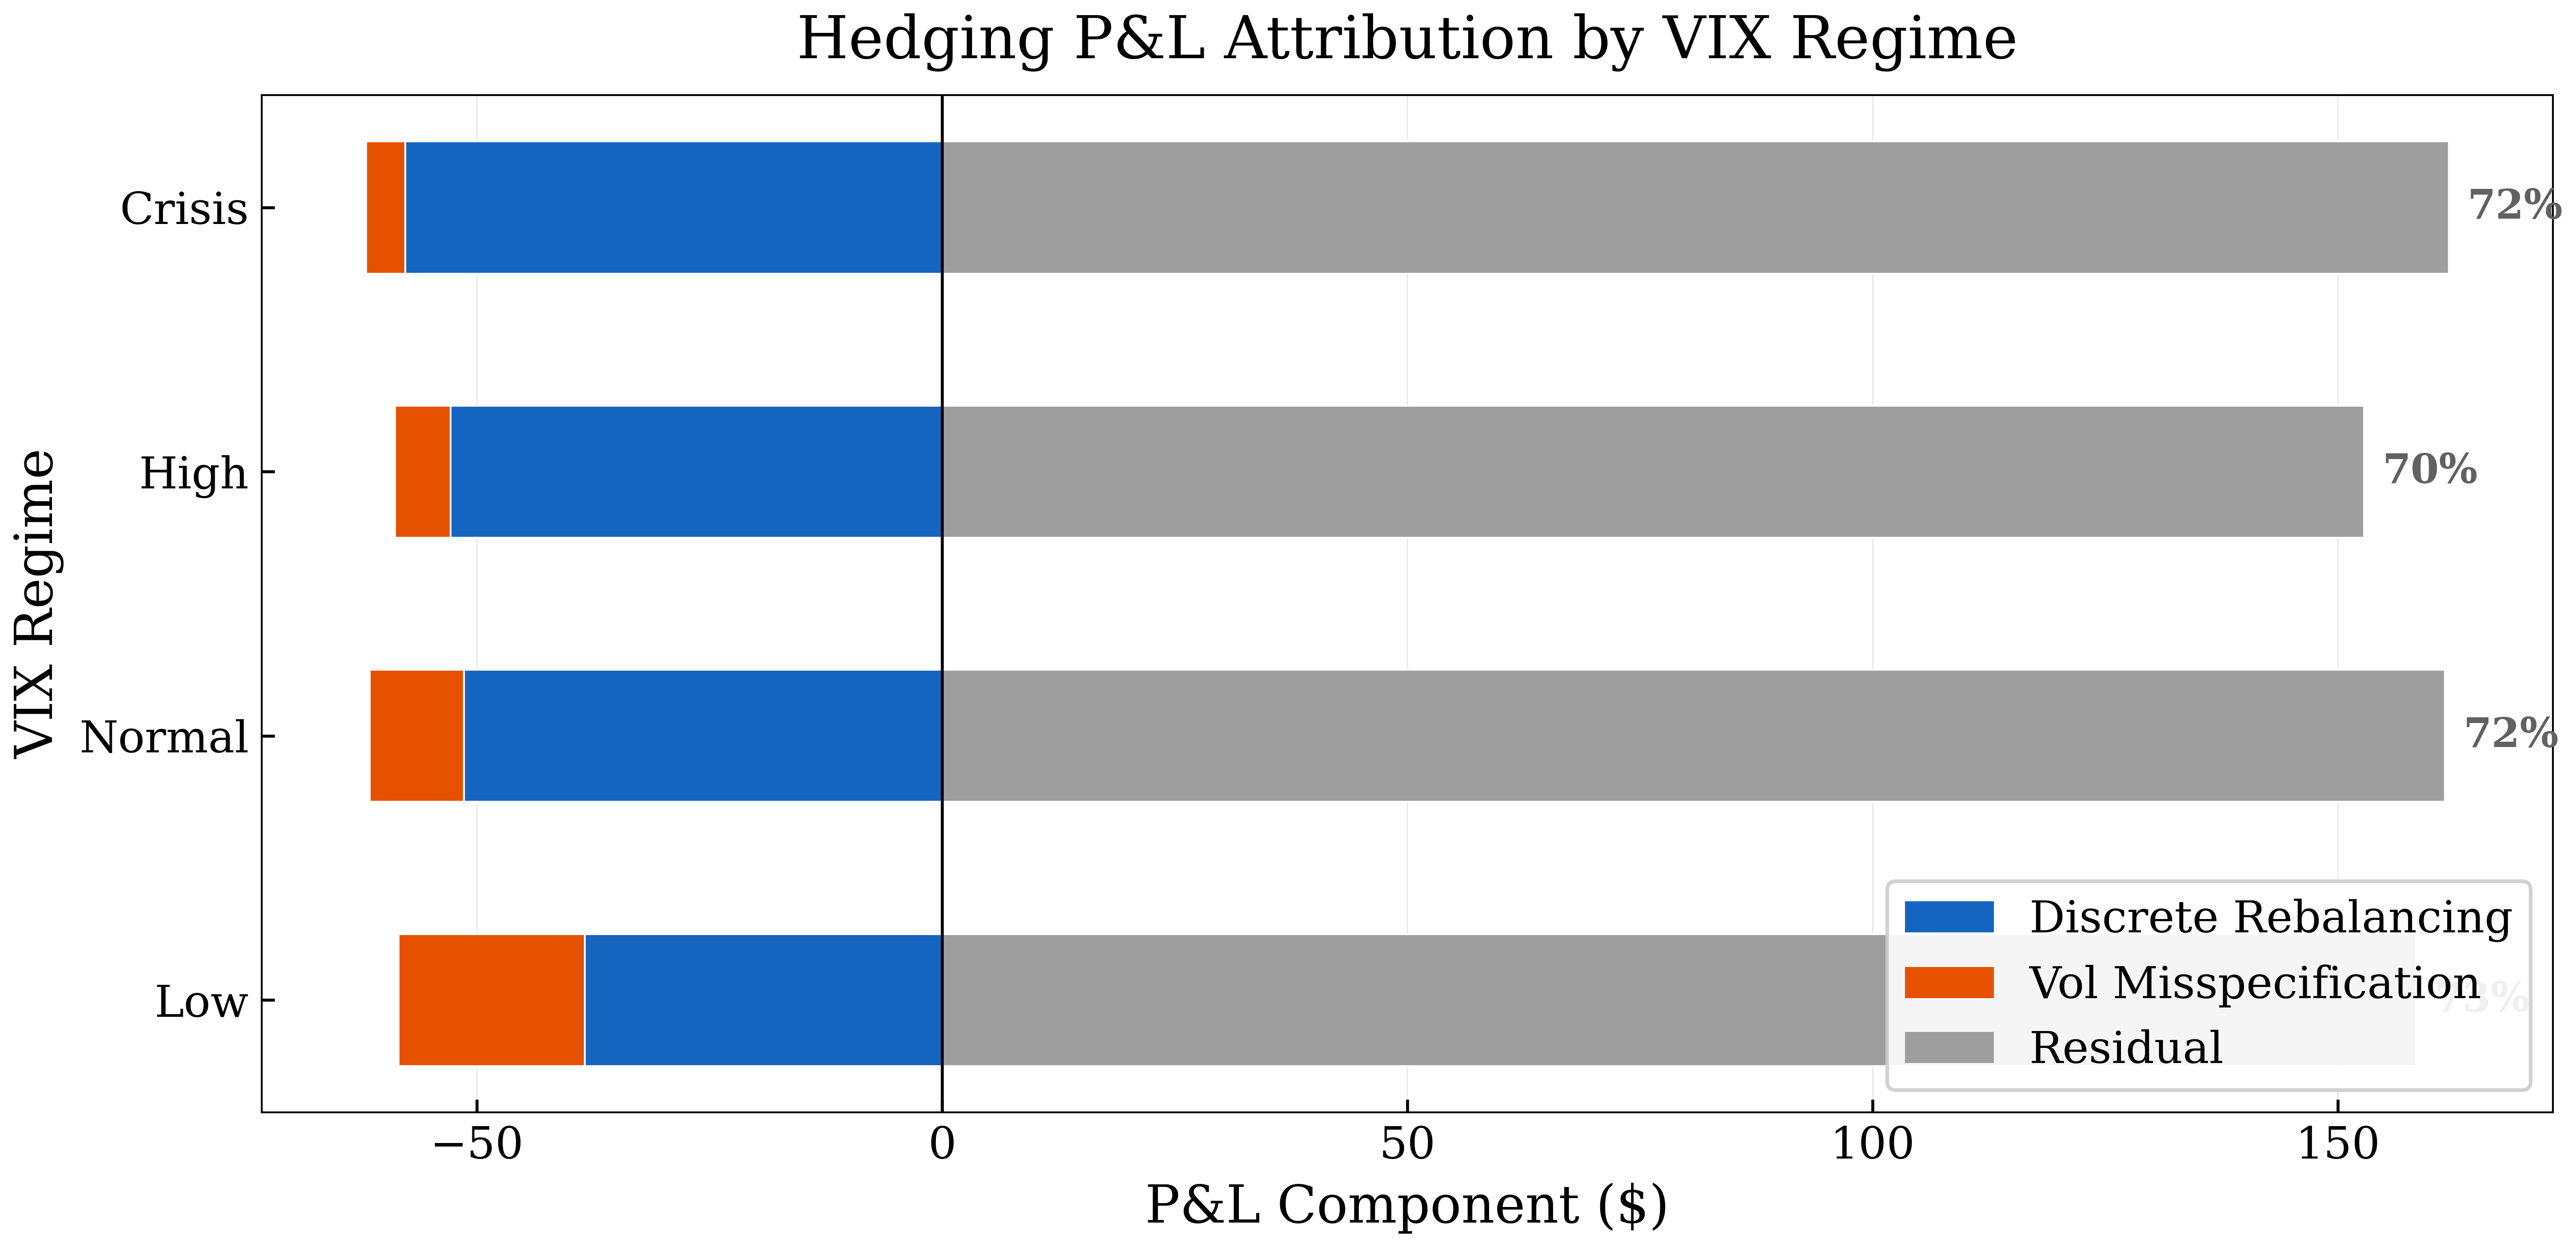
\includegraphics[width=0.85\textwidth]{fig_pnl_simplified.png}

\subsection*{Speaker Notes}
The El Karoui decomposition reveals something important: the biggest source of hedging error is not your volatility input or your rebalancing frequency---it is higher-order effects like vanna, volga, and jumps. These residuals account for 150 to 210 percent of total variance across every VIX regime. Discrete rebalancing contributes negatively, meaning it actually offsets other errors through a diversification effect. This tells you that gamma management matters more than volatility input choice for overall hedging quality. The sum exceeds 100\% because components are correlated---this is a covariance decomposition, not a simple additive breakdown.

\noindent\rule{\textwidth}{0.4pt}

% ═══════════════════════════════════════════════════════════
\section{Slide 10: Why Does the Smile Hurt?}

\subsection*{On-Slide Content}
\begin{enumerate}[nosep]
  \item \textbf{Calibration noise} --- 5-parameter optimization adds estimation error to every delta
  \item \textbf{Interpolation artifacts} --- calibrating every 5th day introduces stale smile information
  \item \textbf{Noise $>$ Signal} --- for most strikes, calibration error outweighs smile information content
  \item \textbf{Exception:} OTM calls, where smile slope is steepest and signal dominates
\end{enumerate}

\subsection*{Figure}
None (text slide).

\subsection*{Speaker Notes}
Why does the smile hurt? Three reasons. First, every SVI calibration introduces noise---you are estimating five parameters from a noisy cross-section of option prices. Flat ATM implied vol has zero calibration error by construction. Second, I calibrate every fifth trading day and interpolate between, so some smile information is stale by the time it reaches the hedge. Third, and most fundamentally, for most strikes the calibration noise simply outweighs the signal. The smile adds information, but it also adds noise, and the noise wins for ATM and OTM put strikes. The exception is OTM calls, where the smile slope is steep enough that the information content dominates. This suggests that daily SVI calibration or SSVI---the arbitrage-free variant---could improve results.

\noindent\rule{\textwidth}{0.4pt}

% ═══════════════════════════════════════════════════════════
\section{Slide 11: Practitioner Takeaway}

\subsection*{On-Slide Content}
\begin{itemize}[nosep]
  \item Match your vol input to what you are hedging
  \item OTM Calls $\to$ SVI Surface IV (+6--12\%)
  \item OTM Puts $\to$ CC Realized Vol (+21--48\%)
  \item ATM $\to$ Flat BSM IV
  \item VIX $\geq$ 35 $\to$ Focus on gamma management
\end{itemize}

\subsection*{Figure}
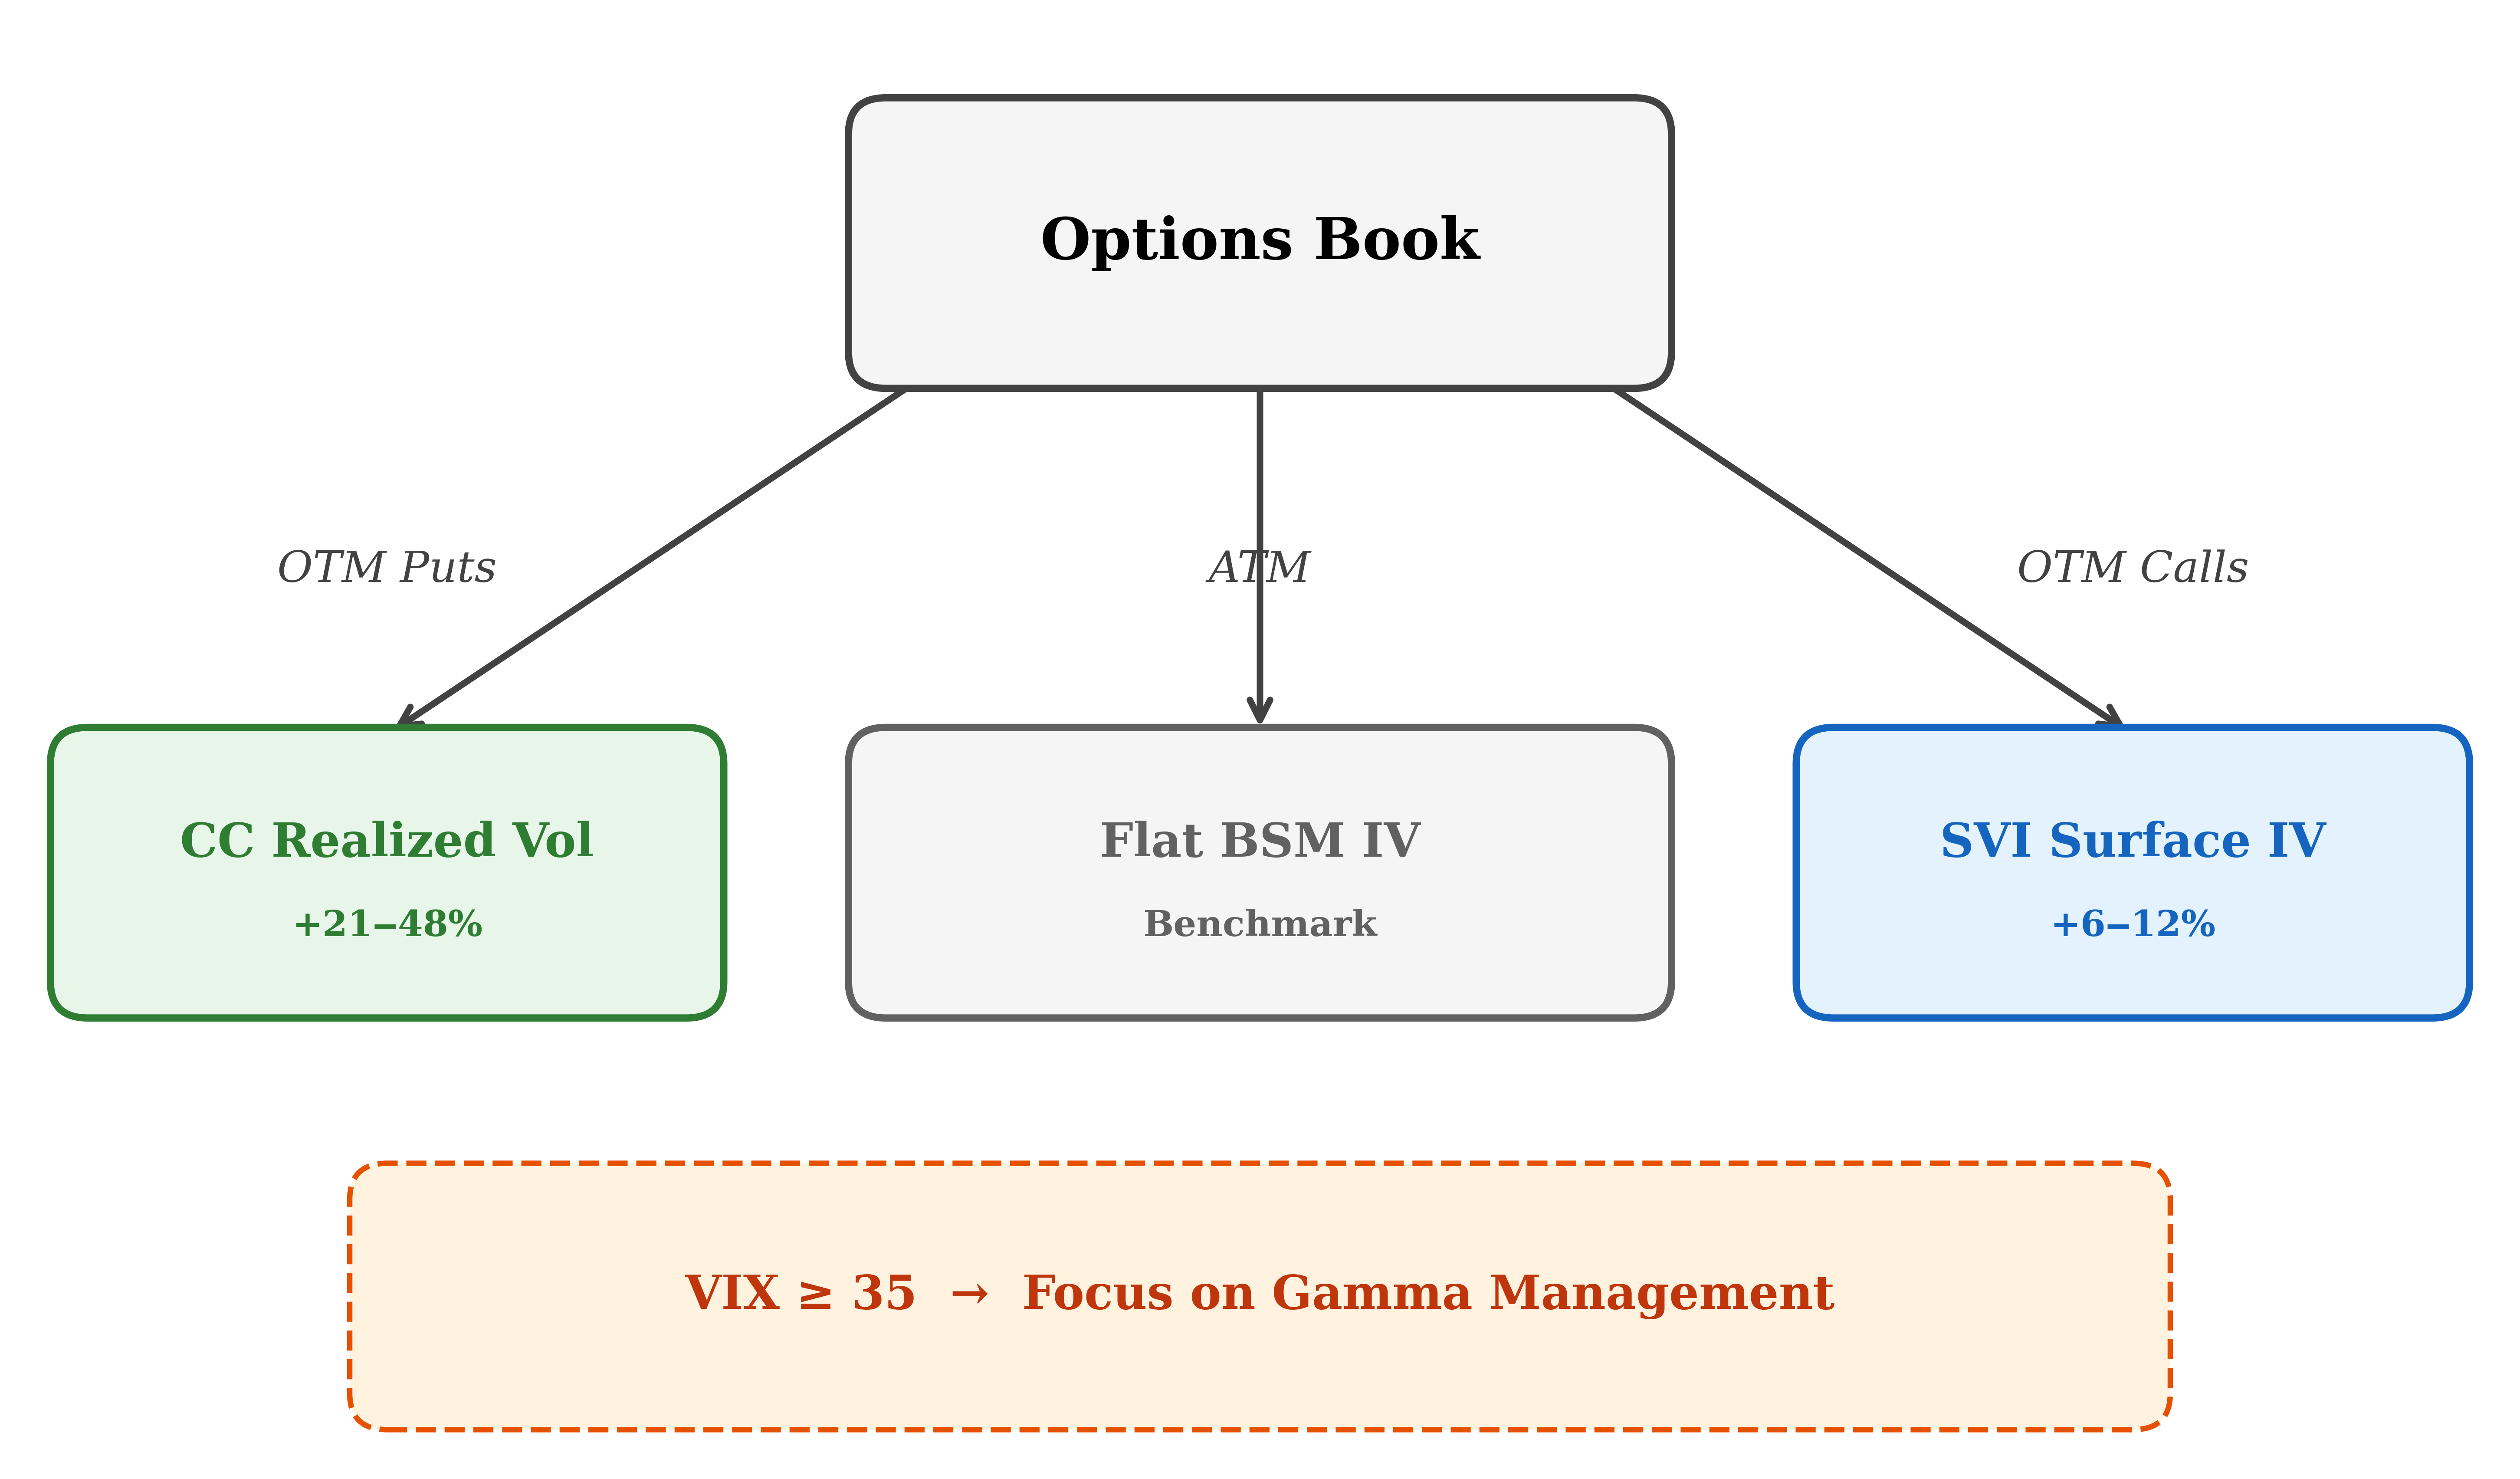
\includegraphics[width=0.85\textwidth]{fig_decision_flowchart.png}

\subsection*{Speaker Notes}
So the practical takeaway is: do not use one volatility for everything. Use SVI for your OTM call book---that is where the smile information actually helps. Use close-to-close realized vol for OTM puts, where the skew premium biases implied-vol deltas. For ATM options, flat BSM is fine---you are not leaving money on the table. And in crisis periods when VIX is above 35, do not overthink the volatility input---focus your energy on managing gamma exposure, because that is where 150-plus percent of your hedging error variance is coming from. A desk hedging \$1B notional could see 5--8\% lower VaR from this conditional approach.

\noindent\rule{\textwidth}{0.4pt}

% ═══════════════════════════════════════════════════════════
\section{Slide 12: Thank You}

\subsection*{On-Slide Content}
\begin{itemize}[nosep]
  \item Zaid Annigeri
  \item \texttt{ma.zaid@rutgers.edu}
  \item Master of Quantitative Finance, Rutgers Business School
  \item GitHub: \texttt{github.com/zaid282802/options-pricing-hedging}
  \item Full thesis and code available upon request
\end{itemize}

\subsection*{Figure}
None.

\subsection*{Speaker Notes}
Thank you for your attention. I am happy to discuss methodology details, walk through the data pipeline, or talk about extensions---including intraday rebalancing, stochastic volatility hedging, or regime-switching models. The full thesis and all code are available on GitHub. I am also working on a statistical arbitrage project that uses the VIX regime classification from this thesis as a feature for trade signal filtering. I welcome your questions.

\end{document}
